% ==================================================================
%  徐森林、金亚东、薛春华《数学分析》（第三册）
%  S13.1  函数项级数的一致收敛
%  源：原书印刷页 77-100（PDF 物理页 83-106）
%  底本：PaddleOCR-VL-1.6，见 chapters/_ch13_13_1_raw.md
%  约定：全西文标点；行间公式用一对方括号；多行公式用 align/aligned；
%        跨册引用一律 \extref；数学模式内的中文必须包 \text{}
%  插图：图 13.1.1、13.1.2 原生 TikZ 绘制（禁用位图）
%  已订正的 OCR 错误与原书照录清单见 tools/_make_ch13_1a.py 头部说明
% ==================================================================
\section{函数项级数的一致收敛}\label{sec:13.1}

在数项级数的基础上, 我们来研究函数项级数.

\begin{definition}\label{def:13.1.1}
设 $u_{n}(x)$ ($n\in\mathbb{N}$) 为定义在集合 $J\subset\mathbb{R}$ 上的函数列. 固定 $x\in J$, $\sum_{n=1}^{\infty}u_{n}(x)$ 为一个数项级数. 当 $x$ 在 $J$ 中变动时, 称 $\sum_{n=1}^{\infty}u_{n}(x)$ 为 $J$ 上的一个函数项级数. $S_{n}(x)=\sum_{k=1}^{n}u_{k}(x)$ 称为该函数项级数的第 $n$ 个部分和.
\end{definition}

如果 $x\in J$, 级数 $\sum_{n=1}^{\infty}u_{n}(x)=\lim\limits_{n\to+\infty}S_{n}(x)$ 收敛, 则称 $x$ 为该函数项级数的收敛点, 或函数项级数在 $x$ 点处收敛; 如果 $x\in J$, 级数 $\sum_{n=1}^{\infty}u_{n}(x)$ 发散, 则称 $x$ 为该函数项级数的发散点, 或函数项级数在 $x$ 点处发散.

$\sum_{n=1}^{\infty}u_{n}(x)$ 的收敛点的集合称为该函数项级数的收敛点集, 记为 $I$; $\sum_{n=1}^{\infty}u_{n}(x)$ 的发散点的集合称为该函数项级数的发散点集.

于是, $\forall x\in I$ (收敛点集), 级数 $\sum_{n=1}^{\infty}u_{n}(x)$ 都有一个确定的和
\[
  S(x)=\lim_{n\to+\infty}S_{n}(x)=\lim_{n\to+\infty}\sum_{k=1}^{n}u_{k}(x).
\]
因此, 它确定了 $I$ 上的一个函数, 称为该函数项级数的和函数, 即 $S(x)=\sum_{n=1}^{\infty}u_{n}(x)$, $x\in I$.

\begin{example}\label{ex:13.1.1}
求函数项级数 $x^{1}+\sum_{n=2}^{\infty}(x^{n}-x^{n-1})$ 的收敛点集. 并研究其和函数的连续性与可导性.
\end{example}

\begin{proof}
因为
\[
  S(x)=\lim_{n\to+\infty}S_{n}(x)=\lim_{n\to+\infty}x^{n}=\begin{cases}
    0, & |x|<1,\\
    1, & x=1,\\
    +\infty, & x>1,\\
    \text{无极限}, & x=-1,\\
    \infty, & x<-1,
\end{cases}
\]
所以收敛点集为 $(-1,1]$.

显然, $x^{1}$, $x^{n}-x^{n-1}$ 在 $(-1,1]$ 上都连续、可导, 但和函数 $S(x)=x^{1}+\sum_{n=2}^{\infty}(x^{n}-x^{n-1})$ 在 $x=1$ 处不连续, 当然也不可导. 换句话说, $S_{n}(x)=x^{n}$ 都在 $(-1,1]$ 上连续、可导, 但极限函数 $S(x)$ 在 $x=1$ 处不连续, 当然也不可导.

换一种方式可表达为
\[
  \begin{aligned}
    \lim_{x\to1^{-}}\sum_{k=1}^{\infty}u_{k}(x)&=\lim_{x\to1^{-}}S(x)=\lim_{x\to1^{-}}0=0\neq1\\
    &=S(1)=\sum_{k=1}^{\infty}u_{k}(1)=\sum_{k=1}^{\infty}\lim_{x\to1^{-}}u_{k}(x),
  \end{aligned}
\]
\[
  \begin{aligned}
    \left(\sum_{k=1}^{\infty}u_{k}(x)\right)'\bigg|_{x=1}&=S'(1)\neq\lim_{n\to+\infty}S_{n}'(1)\\
    &=\lim_{n\to+\infty}\sum_{k=1}^{n}u_{k}'(1)=\sum_{k=1}^{\infty}u_{k}'(1).
  \end{aligned}
\]
即在 $x=1$ 处不能逐项取极限, 不能逐项求导.
\end{proof}

\begin{example}\label{ex:13.1.2}
求函数项级数 $\sum_{n=0}^{\infty}x^{n}$ 的收敛点集与发散点集.
\end{example}

\begin{proof}
从
\[
  \sum_{n=0}^{\infty}x^{n}=\begin{cases}
    \lim\limits_{n\to+\infty}\sum\limits_{k=0}^{n-1}x^{k}=\lim\limits_{n\to+\infty}\frac{1-x^{n}}{1-x}=\frac{1-0}{1-x}=\frac{1}{1-x}, & |x|<1,\\
    \lim\limits_{n\to+\infty}\sum\limits_{k=0}^{n-1}1=\lim\limits_{n\to+\infty}n=+\infty, & x=1,\\
    \lim\limits_{n\to+\infty}\sum\limits_{k=0}^{n-1}(-1)^{k}=\lim\limits_{n\to+\infty}\frac{1+(-1)^{n-1}}{2}\text{ 不存在}, & x=-1,\\
    \lim\limits_{n\to+\infty}\frac{1-x^{n}}{1-x}=+\infty, & x>1,\\
    \lim\limits_{n\to+\infty}\frac{1-x^{n}}{1-x}=\infty, & x<-1
\end{cases}
\]
可知, 该函数项级数 $\sum_{n=0}^{\infty}x^{n}$ 的收敛点集为 $(-1,1)$, 而发散点集为 $(-\infty,-1]\cup[1,+\infty)$.
\end{proof}

\begin{example}\label{ex:13.1.3}
求函数项级数 $\sum_{n=1}^{\infty}\frac{x^{n}}{1+x^{n}}$ 的收敛点集与发散点集.
\end{example}

\begin{proof}
显然, 当 $x=-1$, $n$ 为奇数时 $\frac{x^{n}}{1+x^{n}}$ 无意义; 而每个函数 $\frac{x^{n}}{1+x^{n}}$ 当 $x\neq-1$ 时都有意义. 由于 $n\to+\infty$, 有
\[
  \frac{|u_{n+1}(x)|}{|u_{n}(x)|}=\left|\frac{x(1+x^{n})}{1+x^{n+1}}\right|\to\begin{cases}
    \left|\frac{x(1+0)}{1+0}\right|=|x|<1, & |x|<1,\\
    1, & |x|\geqslant1,\ x\neq-1,
\end{cases}
\]
故当 $|x|<1$ 时, 根据 $d'$Alembert 判别法的极限形式, $\sum_{n=1}^{\infty}\frac{x^{n}}{1+x^{n}}$ 绝对收敛; 又当 $|x|>1$ 时,
\[
  u_{n}(x)=\frac{x^{n}}{1+x^{n}}=\frac{1}{\frac{1}{x^{n}}+1}\to\frac{1}{0+1}=1\quad(n\to+\infty).
\]
根据定理~\ref{thm:12.1.2}, $\sum_{n=1}^{\infty}\frac{x^{n}}{1+x^{n}}$ 发散; 当 $x=1$ 时,
\[
  u_{n}(x)=\frac{1}{2}\to\frac{1}{2}\neq0\quad(n\to+\infty),
\]
再根据定理~\ref{thm:12.1.2} 知道, $\sum_{n=1}^{\infty}\frac{x^{n}}{1+x^{n}}$ 也发散. 由此得到函数项级数 $\sum_{n=1}^{\infty}\frac{x^{n}}{1+x^{n}}$ 的收敛点集为 $(-1,1)$; 发散点集为 $(-\infty,-1]\cup[1,+\infty)$.
\end{proof}

\begin{example}\label{ex:13.1.4}
设 $u_{1}(x)=2x\mathrm{e}^{-x^{2}}$, $u_{n}(x)=2n^{2}x\mathrm{e}^{-n^{2}x^{2}}-2(n-1)^{2}x\mathrm{e}^{-(n-1)^{2}x^{2}}$, $n\geqslant2$. 证明:
\[
  \int_{0}^{1}\sum_{k=1}^{\infty}u_{k}(x)\mathrm{d}x\neq\sum_{k=1}^{\infty}\int_{0}^{1}u_{k}(x)\mathrm{d}x,
\]
即积分号与求和号不能交换, 或不能逐项积分.
\end{example}

\begin{proof}
在 $[0,1]$ 上, 考虑 $\sum_{n=1}^{\infty}u_{n}(x)$ 的部分和函数列
\[
  S_{n}(x)=2n^{2}x\mathrm{e}^{-n^{2}x^{2}},\quad n=1,2,\cdots,
\]
显然
\[
  S(x)=\lim_{n\to+\infty}S_{n}(x)=\lim_{n\to+\infty}2n^{2}x\mathrm{e}^{-n^{2}x^{2}}=0.
\]
因而
\[
  \lim_{n\to+\infty}\int_{0}^{1}S_{n}(x)\mathrm{d}x=\lim_{n\to+\infty}\int_{0}^{1}2n^{2}x\mathrm{e}^{-n^{2}x^{2}}\mathrm{d}x=\lim_{n\to+\infty}\left(-\mathrm{e}^{-n^{2}x^{2}}\right)\Big|_{0}^{1}
\]
\[
  \begin{aligned}
    &=\lim_{n\to+\infty}(1-\mathrm{e}^{-n^{2}})=1\neq0=\int_{0}^{1}0\mathrm{d}x=\int_{0}^{1}S(x)\mathrm{d}x\\
    &=\int_{0}^{1}\lim_{n\to+\infty}S_{n}(x)\mathrm{d}x.
  \end{aligned}
\]
它相当于
\[
  \begin{aligned}
    \sum_{k=1}^{\infty}\int_{0}^{1}u_{k}(x)\mathrm{d}x&=\lim_{n\to+\infty}\sum_{k=1}^{n}\int_{0}^{1}u_{k}(x)\mathrm{d}x=\lim_{n\to+\infty}\int_{0}^{1}\sum_{k=1}^{n}u_{k}(x)\mathrm{d}x\\
    &=\lim_{n\to+\infty}\int_{0}^{1}S_{n}(x)\mathrm{d}x\neq\int_{0}^{1}\lim_{n\to+\infty}S_{n}(x)\mathrm{d}x=\int_{0}^{1}\sum_{k=1}^{\infty}u_{k}(x)\mathrm{d}x.
  \end{aligned}
\]
\end{proof}

\begin{example}\label{ex:13.1.5}
设 $u_{n}(x)=nx(1-x^{2})^{n}-(n-1)x(1-x^{2})^{n-1}$, $n=1,2,\cdots$. 证明:
\[
  \int_{0}^{1}\sum_{n=1}^{\infty}u_{k}(x)\mathrm{d}x\neq\sum_{n=1}^{\infty}\int_{0}^{1}u_{n}(x)\mathrm{d}x,
\]
即积分号与求和号不能交换, 或不能逐项积分.
\end{example}

\begin{proof}
显然, $u_{n}(x)$ 在 $[0,1]$ 上连续, 故它在 $[0,1]$ 上可积, 且
\[
  \begin{aligned}
    \int_{0}^{1}u_{n}(x)\mathrm{d}x&=\int_{0}^{1}\bigl[nx(1-x^{2})^{n}-(n-1)x(1-x^{2})^{n-1}\bigr]\mathrm{d}x\\
    &=\left[-\frac{n}{2(n+1)}(1-x^{2})^{n+1}+\frac{n-1}{2n}(1-x^{2})^{n}\right]_{0}^{1}\\
    &=0-\left[-\frac{n}{2(n+1)}+\frac{n-1}{2n}\right]=\frac{1}{2n(n+1)}.
  \end{aligned}
\]
另一方面, 由函数项级数的部分和
\[
  \begin{aligned}
    S_{n}(x)&=\sum_{k=1}^{n}u_{k}(x)=\sum_{k=1}^{n}\bigl[kx(1-x^{2})^{k}-(k-1)x(1-x^{2})^{k-1}\bigr]\\
    &=nx(1-x^{2})^{n}=\begin{cases}0, & x=0,1,\\ nx(1-x^{2})^{n}, & 0<x<1\end{cases}\to0\quad(n\to+\infty)
  \end{aligned}
\]
知, 其和函数为
\[
  S(x)=\lim_{n\to+\infty}S_{n}(x)=0,\quad\forall x\in[0,1].
\]
于是
\[
  \sum_{n=1}^{\infty}\int_{0}^{1}u_{n}(x)\mathrm{d}x=\sum_{n=1}^{\infty}\frac{1}{2n(n+1)}=\frac{1}{2}\sum_{n=1}^{\infty}\left(\frac{1}{n}-\frac{1}{n+1}\right)
\]
\[
  \xlongequal{\text{裂项相消}}\frac{1}{2}\neq0=\int_{0}^{1}0\mathrm{d}x=\int_{0}^{1}S(x)\mathrm{d}x=\int_{0}^{1}\sum_{n=1}^{\infty}u_{n}(x)\mathrm{d}x.
\]
\end{proof}

\begin{example}\label{ex:13.1.6}
设 $u_{n}(x)=\mathrm{e}^{-n^{2}x^{2}}-\mathrm{e}^{-(n-1)^{2}x^{2}}$, $n=1,2,\cdots$, $u_{n}(x)$ 在 $[0,1]$ 上可导. 证明:
\[
  \left(\sum_{n=1}^{\infty}u_{n}(x)\right)'\neq\sum_{n=1}^{\infty}u_{n}'(x),
\]
即求导与求和号不能交换, 或不能逐项求导.
\end{example}

\begin{proof}
显然
\[
  \begin{aligned}
    \sum_{n=1}^{\infty}u_{n}'(x)&=\sum_{n=1}^{\infty}\bigl[-2n^{2}x\mathrm{e}^{-n^{2}x^{2}}+2(n-1)^{2}x\mathrm{e}^{-(n-1)^{2}x^{2}}\bigr]\\
    &=\lim_{n\to+\infty}\sum_{k=1}^{n}\bigl[-2k^{2}x\mathrm{e}^{-k^{2}x^{2}}+2(k-1)^{2}x\mathrm{e}^{-(k-1)^{2}x^{2}}\bigr]\\
    &\xlongequal{\text{裂项相消}}\lim_{n\to+\infty}(-2n^{2}x\mathrm{e}^{-n^{2}x^{2}})=\begin{cases}\lim\limits_{n\to+\infty}0=0, & x=0,\\ 0, & x\in(0,1]\end{cases}\\
    &=0\neq\left(\sum_{n=1}^{\infty}u_{n}(x)\right)'.
  \end{aligned}
\]
事实上
\[
  \begin{aligned}
    S(x)&=\sum_{n=1}^{\infty}u_{n}(x)=\lim_{n\to+\infty}\sum_{k=1}^{n}u_{k}(x)=\lim_{n\to+\infty}\sum_{k=1}^{n}\bigl[\mathrm{e}^{-k^{2}x^{2}}-\mathrm{e}^{-(k-1)^{2}x^{2}}\bigr]\\
    &\xlongequal{\text{裂项相消}}\lim_{n\to+\infty}(\mathrm{e}^{-n^{2}x^{2}}-1)=\begin{cases}0, & x=0,\\ -1, & 0<x\leqslant1,\end{cases}
  \end{aligned}
\]
它在 $x=0$ 点处不连续, 当然不可导.
\end{proof}

\begin{example}\label{ex:13.1.7}
设 $\mathbb{Q}=\{r_{1},r_{2},\cdots,r_{n},\cdots\}$ 是 $[0,1]$ 上的全体有理数, 在 $[0,1]$ 上定义
\[
  S_{n}(x)=\begin{cases}1, & x=r_{1},r_{2},\cdots,r_{n},\\ 0, & x\text{ 为其他值},\end{cases}\qquad
  S(x)=\begin{cases}1, & x\text{ 为有理数},\\ 0, & x\text{ 为无理数}.\end{cases}
\]
显然, $\lim\limits_{n\to+\infty}S_{n}(x)=S(x)$. 对于每一个固定的 $n\in\mathbb{N}$, $S_{n}(x)$ 在 $[0,1]$ 上是 Riemann 可积的, 但 $S(x)$ 在 $[0,1]$ 上非 Riemann 可积. 当然,
\[
  \int_{0}^{1}S(x)\mathrm{d}x=\lim_{n\to+\infty}\int_{0}^{1}S_{n}(x)\mathrm{d}x
\]
更不成立, 即极限号与积分号不可交换.
\end{example}

如果令 $u_{1}(x)=S_{1}(x)$, $u_{n}(x)=S_{n}(x)-S_{n-1}(x)$, $n=2,3,\cdots$, 则 $S_{n}(x)=\sum_{k=1}^{n}u_{k}(x)$, $S(x)=\sum_{k=1}^{\infty}u_{k}(x)=\lim\limits_{n\to+\infty}\sum_{k=1}^{n}u_{k}(x)=\lim\limits_{n\to+\infty}S_{n}(x)$. 因此
\[
  \begin{aligned}
    \int_{0}^{1}\sum_{k=1}^{\infty}u_{k}(x)\mathrm{d}x&=\int_{0}^{1}S(x)\mathrm{d}x\neq\lim_{n\to+\infty}\int_{0}^{1}S_{n}(x)\mathrm{d}x\\
    &=\lim_{n\to+\infty}\int_{0}^{1}\sum_{k=1}^{n}u_{k}(x)\mathrm{d}x=\lim_{n\to+\infty}\sum_{k=1}^{n}\int_{0}^{1}u_{k}(x)\mathrm{d}x=\sum_{n=1}^{\infty}\int_{0}^{1}u_{k}(x)\mathrm{d}x.
  \end{aligned}
\]
此例表明积分号与求和号不能交换, 即不能逐项积分.

经过上述例子的讨论, 我们首先关心的是函数项级数 $\sum_{n=1}^{\infty}u_{n}(x)$ 所确定的和函数 $S(x)$ 是否具有有限和的各种性质? 也就是:

(1) 如果 $\lim\limits_{x\to x_{0}}u_{n}(x)=a_{n}$ ($n=1,2,\cdots$) 是否有
\[
  \lim_{x\to x_{0}}\lim_{n\to+\infty}S_{n}(x)=\lim_{x\to x_{0}}S(x)=\lim_{x\to x_{0}}\sum_{k=1}^{\infty}u_{k}(x)\overset{?}{=}\sum_{k=1}^{\infty}a_{k}=\sum_{k=1}^{\infty}\lim_{x\to x_{0}}u_{n}(x)=\lim_{n\to+\infty}\lim_{x\to x_{0}}S_{n}(x),
\]
即两个极限号能否交换? 或者函数项级数的求和号与极限号能否交换? 即能否逐项求极限? 特别当 $u_{n}(x)$ ($n=1,2,\cdots$) 都在 $x_{0}$ 连续时, 它成为
\[
  \begin{aligned}
    \lim_{x\to x_{0}}S(x)&=\lim_{x\to x_{0}}\sum_{k=1}^{\infty}u_{k}(x)=\sum_{k=1}^{\infty}\lim_{x\to x_{0}}u_{k}(x)=\sum_{k=1}^{\infty}u_{k}(x_{0})\\
    &\quad\left(=\lim_{n\to+\infty}\sum_{k=1}^{n}u_{k}(x_{0})=\lim_{n\to+\infty}S_{n}(x_{0})\right)=S(x_{0}),
  \end{aligned}
\]
即和函数 $S(x)$ 在 $x_{0}$ 仍连续.

(2) 如果 $u_{n}(x)$ ($n=1,2,\cdots$) 都在 $[a,b]$ 上 Riemann 可积, 它们的和函数 $S(x)$ 是否在 $[a,b]$ 上也 Riemann 可积? 如果 $S(x)$ 在 $[a,b]$ 上 Riemann 可积, 等式
\[
  \begin{aligned}
    \int_{a}^{b}\lim_{n\to+\infty}S_{n}(x)\mathrm{d}x&=\int_{a}^{b}S(x)\mathrm{d}x=\int_{a}^{b}\sum_{k=1}^{\infty}u_{k}(x)\mathrm{d}x\\
    &\overset{?}{=}\sum_{k=1}^{\infty}\int_{a}^{b}u_{k}(x)\mathrm{d}x=\lim_{n\to+\infty}\sum_{k=1}^{n}\int_{a}^{b}u_{k}(x)\mathrm{d}x=\lim_{n\to+\infty}\int_{a}^{b}S_{n}(x)\mathrm{d}x
  \end{aligned}
\]
是否成立? 即积分号与极限号能否交换? 或者函数项级数的求和号与积分号能否交换? 即能否逐项求积分?

(3) 如果 $u_{n}(x)$ ($n=1,2,\cdots$) 都在 $[a,b]$ 上可导, $S(x)$ 在 $[a,b]$ 上是否也可导? 等式
\[
  \begin{aligned}
    (\lim_{n\to+\infty}S_{n}(x))'&=S'(x)=\left(\sum_{n=1}^{\infty}u_{k}(x)\right)'\\
    &\overset{?}{=}\sum_{k=1}^{\infty}u_{k}'(x)=\lim_{n\to+\infty}\sum_{k=1}^{n}u_{k}'(x)=\lim_{n\to+\infty}S_{n}'(x)
  \end{aligned}
\]
是否成立? 即求导与极限号能否交换? 或者函数项级数的求和号与导数运算能否交换? 即能否逐项求导?

以上 (1)、(2)、(3) 可依次简述为
\[
  \begin{aligned}
    &\lim_{x\to x_{0}}\lim_{n\to+\infty}S_{n}(x)=\lim_{n\to+\infty}\lim_{x\to x_{0}}S_{n}(x)\\
    &\quad\text{或}\quad\lim_{x\to x_{0}}\sum_{k=1}^{\infty}u_{k}(x)\xlongequal{\text{逐项求极限}}\sum_{k=1}^{\infty}\lim_{x\to x_{0}}u_{k}(x)\text{;}\\
    &\int_{a}^{b}S(x)\mathrm{d}x=\int_{a}^{b}\lim_{n\to+\infty}S_{n}(x)\mathrm{d}x=\lim_{n\to+\infty}\int_{a}^{b}S_{n}(x)\mathrm{d}x\\
    &\quad\text{或}\quad\int_{a}^{b}\sum_{k=1}^{\infty}u_{k}(x)\mathrm{d}x\xlongequal{\text{逐项求积分}}\sum_{k=1}^{\infty}\int_{a}^{b}u_{k}(x)\mathrm{d}x\text{;}\\
    &S'(x)=(\lim_{n\to+\infty}S_{n}(x))'=\lim_{n\to+\infty}S_{n}'(x)\quad\text{或}\quad\left(\sum_{k=1}^{\infty}u_{k}(x)\right)'\xlongequal{\text{逐项求导}}\sum_{k=1}^{\infty}u_{k}'(x)
  \end{aligned}
\]
是否成立? 回答是否定的. 例~\ref{ex:13.1.1}, 例~\ref{ex:13.1.4}$\sim$例~\ref{ex:13.1.7} 就是所需的反例. 进而, 自然会问, 应附加什么条件, 上述各式一定成立. 这是使等式成立的充分条件. 思来想去, 19 世纪许多著名的数学家发现, 为给出充分条件必须引进比函数项级数收敛更强的一致收敛的重要概念.

根据函数项级数 $\sum_{n=1}^{\infty}u_{n}(x)$ 与部分和函数列 $\{S_{n}(x)\}$ 之间的对偶关系, 自然可将\extref{定义 6.3.1} 中函数列一致收敛的概念与性质翻译成函数项级数 $\sum_{n=1}^{\infty}u_{n}(x)$ 的一致收敛性概念与性质.

设 $\{f_{n}(x)\}$ 为定义在 $I\subseteq\mathbb{R}$ 上的一个函数列. 对于 $x_{0}\in I$, 如果数列 $\{f_{n}(x_{0})\}$ 收敛, 就称函数列 $\{f_{n}(x)\}$ 在 $x_{0}$ 点收敛. 如果 $\{f_{n}(x)\}$ 在 $I$ 中每点都收敛, 就称 $\{f_{n}(x)\}$ 在 $I$ 上收敛或 $I$ 上逐点收敛. 一般来说, 这些数列收敛的快慢是不一致的, 有的收敛的快些, 有的慢些. 用 $\varepsilon$-$N$ 的语言, $\forall x_{0}\in I$, $\forall\varepsilon>0$, $\exists N=N(x_{0},\varepsilon)\in\mathbb{N}$, 当 $n>N$ 时, 就有
\[
  |f_{n}(x_{0})-f(x_{0})|<\varepsilon.
\]
这里 $N=N(x_{0},\varepsilon)$ 不仅与 $\varepsilon$ 有关, 也与 $x_{0}$ 有关. 对于同一个 $\varepsilon>0$, 不同的 $x_{0}$ 所要求的 $N(x_{0},\varepsilon)$ 值可以相差很大.

\begin{example}\label{ex:13.1.8}
(1) 设 $f_{n}(x)=x^{n}$, $x\in(0,1)$. 显然
\[
  f(x)=\lim_{n\to+\infty}f_{n}(x)=\lim_{n\to+\infty}x^{n}=0.
\]
于是, $\forall\varepsilon\in(0,1)$, 取 $N=N(x,\varepsilon)=\left[\frac{\ln\varepsilon}{\ln x}\right]$, 当 $n>N(x,\varepsilon)=\left[\frac{\ln\varepsilon}{\ln x}\right]$ 时, 有 $n>\frac{\ln\varepsilon}{\ln x}$, 且
\[
  |f_{n}(x)-f(x)|=|x^{n}-0|=x^{n}<\varepsilon.
\]
对于不同的 $x$, 相应的 $N(x,\varepsilon)$ 就很不一样. 例如: 取 $\varepsilon=10^{-100}$, $x=10^{-10}$, $10^{-4}$, $10^{-1}$ 就分别有 $N(x,\varepsilon)=\left[\frac{\ln\varepsilon}{\ln x}\right]=10$, 25, 100. 由此可见, 当 $x$ 越靠近原点, $\{x^{n}\}$ 收敛于 $0$ 的速度越快. 那么, 对任意给定的 $\varepsilon>0$, 能否找到一个与 $x$ 无关的 $N=N(\varepsilon)$, 只要 $n>N$, 对 $(0,1)$ 中任意 $x$ 都有 $x^{n}<\varepsilon$ 呢? 容易知道, 这样的 $N$ 是不存在的. (反证) 假设这样的 $N=N(\varepsilon)$ 存在, 则当 $n>N$ 时, 恒有 $x^{n}<\varepsilon$. 取 $x=\varepsilon^{\frac{1}{n}}$, 便得到不等式
\[
  \varepsilon=(\varepsilon^{\frac{1}{n}})^{n}=x^{n}<\varepsilon,
\]
矛盾 (或者设 $\varepsilon\in(0,1)$, 由于 $x^{n}<\varepsilon$, $\forall x\in(0,1)$, 令 $x\to1^{-}$ 得到 $1\leqslant\varepsilon<1$, 矛盾).

实际上, 固定 $\varepsilon>0$, 就有
\[
  \lim_{x\to1^{-}}N(x,\varepsilon)=\lim_{x\to1^{-}}\left[\frac{\ln\varepsilon}{\ln x}\right]=+\infty,
\]
这也说明不存在与 $x$ 无关的 $N=N(\varepsilon)$.

(2) 设 $f_{n}(x)=\frac{1}{n+x}$, $n=1,2,\cdots$. 显然, $\forall x\in(0,1)$, 都有 $f(x)=\lim\limits_{n\to+\infty}f_{n}(x)=0$.
\end{example}

于是, $\forall\varepsilon>0$, 取 $N=N(\varepsilon)=\left[\frac{1}{\varepsilon}\right]$, 当 $n>N$ 时, 有 $n>\frac{1}{\varepsilon}$, 且
\[
  |f_{n}(x)-f(x)|=\left|\frac{1}{n+x}-0\right|=\frac{1}{n+x}<\frac{1}{n}<\varepsilon,\quad\forall x\in(0,1).
\]
显然, 这时的 $N=N(\varepsilon)=\left[\frac{1}{\varepsilon}\right]$ 只与 $\varepsilon$ 有关, 而与 $x$ 无关!

以上两例, 同时都在 $(0,1)$ 上收敛, 然而却有似乎很微小但又是非常重要的差别: 在给定正数 $\varepsilon$ 以后, 前者对于每一个 $x\in(0,1)$, 都有相应的 $N(x,\varepsilon)$, 但却找不到一个与 $x$ 无关的 $N$; 后者则有这样的 $N$. 因此, 后者比前者多满足了一个条件: 存在与 $x$ 无关的 $N$. 这个条件对于上面提出的 (1)、(2)、(3) 成立具有实质性的作用. 因此, 有必要在原来的收敛概念的基础上建立一个更强的一致收敛概念. 回顾一下\extref{定义 6.3.1}, 它就是下面的定义.

\begin{definition}\label{def:13.1.2}
设函数列 $\{f_{n}(x)\}$ 在 $I\subset\mathbb{R}$ 上收敛于 $f(x)$. 如果 $\forall\varepsilon>0$, $\exists N=N(\varepsilon)\in\mathbb{N}$ ($N(\varepsilon)$ 只与 $\varepsilon$ 有关而与 $x\in I$ 无关), 使得当 $n>N=N(\varepsilon)$ 时, 有
\[
  |f_{n}(x)-f(x)|<\varepsilon,\quad\forall x\in I,
\]
即 $f(x)-\varepsilon<f_{n}(x)<f(x)+\varepsilon$, 则称函数列 $\{f_{n}(x)\}$ 在 $I$ 上一致收敛于函数 $f(x)$ (\cref{fig:13.1.1}). 并简记为
\[
  f_{n}(x)\rightrightarrows f(x)\quad(n\to+\infty),\ x\in I.
\]
\end{definition}

从几何上看, $y=f_{n}(x)$ ($n=1,2,\cdots$) 表示一列曲线, 所谓 $\{f_{n}(x)\}$ 一致收敛于 $f(x)$, 就是从某个足标 $N=N(\varepsilon)$ 之后, 所有的曲线
\[
  y=f_{n}(x),\quad n=N+1,N+2,\cdots
\]
全部落入条形区域 $f(x)-\varepsilon<y<f(x)+\varepsilon$ (\cref{fig:13.1.1}) 之中.

\begin{figure}[htbp]
  \centering
  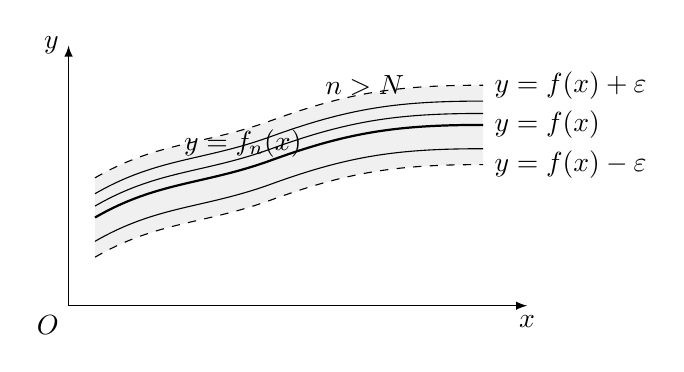
\begin{tikzpicture}[>=latex, scale=1.12]
    % 条形区域 f(x)-eps < y < f(x)+eps
    \fill[black!6] (0.4,1.00) to[out=30,in=200] (2.4,1.65) to[out=20,in=180] (4.80,2.05)
      -- (4.80,2.95) to[out=180,in=20] (2.4,2.55) to[out=200,in=30] (0.4,1.90) -- cycle;
    % 上、下边界（虚线）
    \draw[dashed] (0.4,1.90) to[out=30,in=200] (2.4,2.55) to[out=20,in=180] (4.80,2.95);
    \draw[dashed] (0.4,1.00) to[out=30,in=200] (2.4,1.65) to[out=20,in=180] (4.80,2.05);
    % 极限函数 y=f(x)
    \draw[thick] (0.4,1.45) to[out=30,in=200] (2.4,2.10) to[out=20,in=180] (4.80,2.50);
    % N 之后的曲线 y=f_n(x)
    \draw[thin] (0.4,1.18) to[out=30,in=200] (2.4,1.83) to[out=20,in=180] (4.80,2.23);
    \draw[thin] (0.4,1.58) to[out=30,in=200] (2.4,2.23) to[out=20,in=180] (4.80,2.63);
    \draw[thin] (0.4,1.72) to[out=30,in=200] (2.4,2.37) to[out=20,in=180] (4.80,2.77);
    % 坐标轴
    \draw[->] (0.10,0.45) -- (5.30,0.45) node[below] {$x$};
    \draw[->] (0.10,0.45) -- (0.10,3.40) node[left] {$y$};
    \node[below left] at (0.10,0.45) {$O$};
    % 文字标注
    \node[right] at (4.82,2.95) {$y=f(x)+\varepsilon$};
    \node[right] at (4.82,2.50) {$y=f(x)$};
    \node[right] at (4.82,2.05) {$y=f(x)-\varepsilon$};
    \node[above right] at (1.30,2.02) {$y=f_{n}(x)$};
    \node[above right] at (2.90,2.72) {$n>N$};
  \end{tikzpicture}
  \caption{一致收敛的几何意义}\label{fig:13.1.1}
\end{figure}

根据这个定义, 函数列 $\{x^{n}\}$ 在 $(0,1)$ 上收敛于 $0$, 但不一致收敛于 $0$. 从 \cref{fig:13.1.2} 可以看出, 不论 $n$ 多大, 曲线 $y=x^{n}$ 永远不会全部落入条形区域 $-\varepsilon<y<\varepsilon$ 之中, 其中 $\varepsilon\in(0,1)$. 因而 $\{x^{n}\}$ 在 $(0,1)$ 上不是一致收敛于 $0$ 的.

\begin{figure}[htbp]
  \centering
  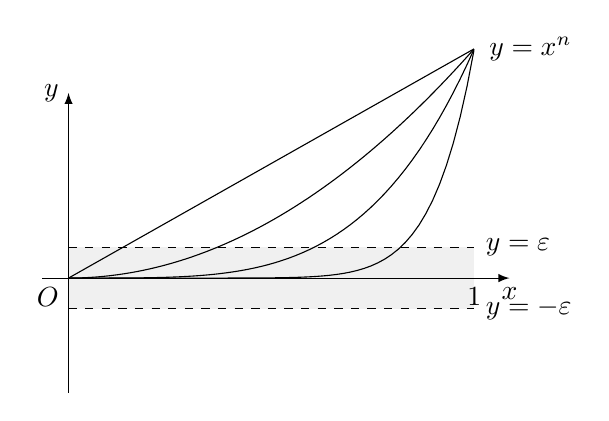
\begin{tikzpicture}[>=latex, scale=1.12]
    % 条形区域 -eps < y < eps
    \fill[black!6] (0,0.35) rectangle (4.60,-0.35);
    \draw[dashed] (0,0.35) -- (4.60,0.35);
    \draw[dashed] (0,-0.35) -- (4.60,-0.35);
    % 曲线 y=x^n (n=1,2,4,10)
    \foreach \n in {1,2,4,10}{
      \draw[thin, domain=0:1, samples=60] plot ({\x*4.60}, {pow(\x,\n)*2.60});
    }
    % 坐标轴
    \draw[->] (-0.30,0) -- (5.00,0) node[below] {$x$};
    \draw[->] (0,-1.30) -- (0,2.10) node[left] {$y$};
    \node[below left] at (0,0) {$O$};
    \node[below] at (4.60,0) {$1$};
    % 文字标注
    \node[right] at (4.62,0.35) {$y=\varepsilon$};
    \node[right] at (4.62,-0.35) {$y=-\varepsilon$};
    \node[right] at (4.66,2.60) {$y=x^{n}$};
  \end{tikzpicture}
  \caption{$\{x^{n}\}$ 在 $(0,1)$ 上不一致收敛}\label{fig:13.1.2}
\end{figure}

而由例~\ref{ex:13.1.8}(2) 的证明知, 函数列 $\left\{\frac{1}{n+x}\right\}$ 在 $(0,1)$ 上一致收敛于 $0$.

像数列的 Cauchy 收敛准则一样, 也有判断函数列是否一致收敛的 Cauchy 准则, 它的优点是无需知道极限函数, 就能判别其是否一致收敛.

\begin{theorem}[函数列一致收敛的 Cauchy 收敛准则]\label{thm:13.1.1}
设 $\{f_{n}(x)\}$ 为 $I\subset\mathbb{R}$ 上的一个函数列, 则以下结论等价:

(1) $\{f_{n}(x)\}$ 在 $I$ 上一致收敛;

(2) $\forall\varepsilon>0$, $\exists N=N(\varepsilon)\in\mathbb{N}$, 当 $n,m>N$ 时, $|f_{m}(x)-f_{n}(x)|<\varepsilon$, $\forall x\in I$;

(3) $\forall\varepsilon>0$, $\exists N=N(\varepsilon)\in\mathbb{N}$, 当 $n>N$ 时, $|f_{n+p}(x)-f_{n}(x)|<\varepsilon$, $\forall x\in I$, $\forall p\in\mathbb{N}$.
\end{theorem}

\begin{proof}
(2) $\Leftrightarrow$ (3) 显然.

(1) $\Rightarrow$ (2) 设 $\{f_{n}(x)\}$ 在 $I$ 上一致收敛于 $f(x)$, 则 $\forall\varepsilon>0$, $\exists N=N(\varepsilon)\in\mathbb{N}$, 当 $n>N$ 时, 有
\[
  |f_{n}(x)-f(x)|<\frac{\varepsilon}{2},\quad\forall x\in I.
\]
于是, 当 $n,m>N$ 时, 有
\[
  |f_{m}(x)-f_{n}(x)|\leqslant|f_{m}(x)-f(x)|+|f(x)-f_{n}(x)|<\frac{\varepsilon}{2}+\frac{\varepsilon}{2}=\varepsilon,\quad\forall x\in I.
\]

(1) $\Leftrightarrow$ (2) 设 (2) 成立, 则 $\forall\varepsilon>0$, $\exists N=N(\varepsilon)\in\mathbb{N}$, 当 $n,m>N$ 时, $|f_{m}(x)-f_{n}(x)|<\frac{\varepsilon}{2}$, $\forall x\in I$. 根据数列的 Cauchy 收敛准则, $\{f_{n}(x)\}$ 在 $I$ 上每点 $x$ 处都收敛, 设其极限函数为 $f(x)$. 在
\[
  |f_{m}(x)-f_{n}(x)|<\frac{\varepsilon}{2}
\]
中令 $m\to+\infty$ 得到
\[
  |f(x)-f_{n}(x)|\leqslant\frac{\varepsilon}{2}<\varepsilon,\quad\forall x\in I.
\]
根据定义~\ref{def:13.1.2}, $\{f_{n}(x)\}$ 在 $I$ 上一致收敛于 $f(x)$.
\end{proof}

\begin{theorem}\label{thm:13.1.2}
函数列 $\{f_{n}(x)\}$ 在 $I\subset\mathbb{R}$ 上一致收敛于 $f(x)$ $\Leftrightarrow$ $\lim\limits_{n\to+\infty}\beta_{n}=0$, 其中 $\beta_{n}=\sup\limits_{x\in I}|f_{n}(x)-f(x)|$.
\end{theorem}

\begin{proof}
($\Rightarrow$) 设 $\{f_{n}(x)\}$ 在 $I$ 上一致收敛, 则 $\forall\varepsilon>0$, $\exists N=N(\varepsilon)\in\mathbb{N}$, 当 $n>N$ 时, 有
\[
  |f_{n}(x)-f(x)|<\frac{\varepsilon}{2},\quad\forall x\in I.
\]
由此得到
\[
  \beta_{n}=\sup_{x\in I}|f_{n}(x)-f(x)|\leqslant\frac{\varepsilon}{2}<\varepsilon,
\]
即 $\lim\limits_{n\to+\infty}\beta_{n}=0$.

($\Leftrightarrow$) 设 $\lim\limits_{n\to+\infty}\beta_{n}=0$, 则 $\forall\varepsilon>0$, $\exists N=N(\varepsilon)\in\mathbb{N}$, 当 $n>N$ 时, $\beta_{n}<\varepsilon$. 有
\[
  |f_{n}(x)-f(x)|\leqslant\sup_{u\in I}|f_{n}(u)-f(u)|\doteq\beta_{n}<\varepsilon,
\]
这就证明了 $\{f_{n}(x)\}$ 在 $I$ 上是一致收敛的.
\end{proof}

\begin{example}\label{ex:13.1.9}
在例~\ref{ex:13.1.8}(1) 中, 由于
\[
  \beta_{n}=\sup_{x\in(0,1)}|f_{n}(x)-f(x)|=\sup_{x\in(0,1)}x^{n}=1\not\to0\quad(n\to+\infty),
\]
故 $f_{n}(x)=x^{n}$ 在 $(0,1)$ 上不一致收敛.
\end{example}

\begin{example}\label{ex:13.1.10}
分别讨论函数列 $f_{n}(x)=\frac{nx}{1+n^{2}x^{2}}$ 在 $(0,1)$ 与 $(1,+\infty)$ 上的一致收敛性.
\end{example}

\begin{proof}
对任意给定的 $x\in(0,+\infty)$, 显然, $f(x)=\lim\limits_{n\to+\infty}f_{n}(x)=\lim\limits_{n\to+\infty}\frac{nx}{1+n^{2}x^{2}}=0$.

(1) 当 $x\in(0,1)$ 时, 由于
\[
  \beta_{n}=\sup_{x\in(0,1)}|f_{n}(x)-f(x)|=\left|f_{n}\left(\frac{1}{n}\right)-f\left(\frac{1}{n}\right)\right|=\frac{1}{2}\not\to0\quad(n\to+\infty),
\]
所以, $\lim\limits_{n\to+\infty}\beta_{n}\neq0$. 根据定理~\ref{thm:13.1.2} 知, $\{f_{n}(x)\}$ 在 $(0,1)$ 上不一致收敛于 $0$.

(2) 当 $x\in(1,+\infty)$ 时, $\forall\varepsilon>0$, 取 $N=N(\varepsilon)>\frac{1}{\varepsilon}$, 当 $n>N$ 时, 有
\[
  |f_{n}(x)-f(x)|=\frac{nx}{1+n^{2}x^{2}}\leqslant\frac{nx}{n^{2}x^{2}}=\frac{1}{nx}<\frac{1}{n}<\frac{1}{N}<\varepsilon,
\]
故 $\{f_{n}(x)\}$ 在 $(1,+\infty)$ 上一致收敛于 $0$. 或者由
\[
  0\leqslant\beta_{n}=\sup_{x\in(1,+\infty)}|f_{n}(x)-f(x)|\leqslant\frac{1}{n}\to0\quad(n\to+\infty)
\]
及夹逼定理得到 $\lim\limits_{n\to+\infty}\beta_{n}=0$. 根据定理~\ref{thm:13.1.2} 知 $\{f_{n}(x)\}$ 在 $(1,+\infty)$ 上一致收敛.
\end{proof}

\begin{example}\label{ex:13.1.11}
讨论函数列
\[
  f_{n}(x)=2n^{2}x\mathrm{e}^{-n^{2}x^{2}},\quad n=1,2,\cdots
\]
在 $[0,1]$ 上的一致收敛性.
\end{example}

\begin{proof}
从例~\ref{ex:13.1.4} 知, $f(x)=\lim\limits_{n\to+\infty}f_{n}(x)=\lim\limits_{n\to+\infty}2n^{2}x\mathrm{e}^{-n^{2}x^{2}}=0$. 由于
\[
  \beta_{n}=\sup_{x\in(0,1)}|f_{n}(x)-f(x)|\geqslant\left|f_{n}\left(\frac{1}{n}\right)-f\left(\frac{1}{n}\right)\right|=2n\mathrm{e}^{-1}\to+\infty\neq0\quad(n\to+\infty),
\]
故 $\lim\limits_{n\to+\infty}\beta_{n}\neq0$. 根据定理~\ref{thm:13.1.2} 推得 $\{f_{n}(x)\}$ 在 $[0,1]$ 上非一致收敛.
\end{proof}

\begin{example}\label{ex:13.1.12}
证明:
\[
  \sum_{n=1}^{\infty}\bigl[\mathrm{e}^{-n^{2}x^{2}}-\mathrm{e}^{-(n-1)^{2}x^{2}}\bigr]
\]
在 $(0,1)$ 中不一致收敛.
\end{example}

\begin{proof}
$S_{n}(x)=\mathrm{e}^{-n^{2}x^{2}}-1$,
\[
  S(x)=\lim_{n\to+\infty}(\mathrm{e}^{-n^{2}x^{2}}-1)=0-1=-1,\quad\forall x\in(0,1).
\]
\[
  \begin{aligned}
    \beta_{n}&=\sup_{x\in(0,1)}|S_{n}(x)-S(x)|=\sup_{x\in(0,1)}\mathrm{e}^{-n^{2}x^{2}}\geqslant\mathrm{e}^{-n^{2}\cdot\frac{1}{n^{2}}}\\
    &=\mathrm{e}^{-1}\not\to0\quad(n\to+\infty),
  \end{aligned}
\]
从而 $\lim\limits_{n\to+\infty}\beta_{n}\neq0$. 根据定理~\ref{thm:13.1.2}, 原函数项级数在 $(0,1)$ 中不一致收敛.
\end{proof}

%  第二部分：定义 13.1.2' 起（生成脚本 tools/_make_ch13_1b.py）
% ==================================================================

% ===== PART-B =====

应用函数项级数与部分和函数列之间的对偶关系, 我们将给出函数项级数的一致收敛及其判别法.

\begin{definitionp}\label{def:13.1.2p}
设 $\sum_{n=1}^{\infty}u_{n}(x)$ 是定义在 $I\subset\mathbb{R}$ 上的函数项级数, $S_{n}(x)=\sum_{k=1}^{n}u_{k}(x)$ 为其部分和. 如果函数列 $\{S_{n}(x)\}$ 在 $I$ 上一致收敛于 $S(x)$, 就称 $\sum_{n=1}^{\infty}u_{n}(x)$ 在 $I$ 上一致收敛于 $S(x)$. 并记 $S(x)=\sum_{n=1}^{\infty}u_{n}(x)$. 用 $\varepsilon$-$N$ 语言表达为: $\forall\varepsilon>0$, $\exists N=N(\varepsilon)\in\mathbb{N}$, 当 $n>N$ 时, 有
\[
  \left|\sum_{k=n+1}^{\infty}u_{k}(x)\right|=\left|\sum_{k=1}^{n}u_{k}(x)-\sum_{k=1}^{\infty}u_{k}(x)\right|=|S_{n}(x)-S(x)|<\varepsilon,\quad\forall x\in I.
\]
\end{definitionp}

% 定理 13.1.1' 排在定理 13.1.2 之后：先把计数器拨回 1（环境内 -1 再自增 -> 13.1.1'），
% 退出后再拨回 2，使下一个普通定理为 13.1.3。
\setcounter{theorem}{1}
\begin{theoremp}[函数项级数一致收敛的 Cauchy 准则]\label{thm:13.1.1p}
以下结论等价:

(1) 函数项级数 $\sum_{n=1}^{\infty}u_{n}(x)$ 在 $I\subset\mathbb{R}$ 上一致收敛;

(2) $\forall\varepsilon>0$, $\exists N=N(\varepsilon)\in\mathbb{N}$, 当 $m>n>N$ 时, 有
\[
  \left|\sum_{k=n+1}^{m}u_{k}(x)\right|<\varepsilon,\quad\forall x\in I;
\]

(3) $\forall\varepsilon>0$, $\exists N=N(\varepsilon)\in\mathbb{N}$, 当 $n>N$ 时, 有
\[
  \left|\sum_{k=n+1}^{n+p}u_{k}(x)\right|<\varepsilon,\quad\forall p\in\mathbb{N},\quad\forall x\in I.
\]
\end{theoremp}
\addtocounter{theorem}{1}

\begin{proof}
(1)
\[
  \begin{aligned}
    &\sum_{n=1}^{\infty}u_{n}(x)\text{ 在 }I\text{ 上一致收敛}\\
    &\Leftrightarrow\{S_{n}(x)\}\text{ 在 }I\text{ 上一致收敛}\\
    &\Leftrightarrow\forall\varepsilon>0,\ \exists N=N(\varepsilon)\in\mathbb{N},\ \text{当 }m\geqslant n>N\text{ 时, 有}\\
    &\qquad|S_{m}(x)-S_{n}(x)|<\varepsilon,\quad\forall x\in I\\
    &\Leftrightarrow(2)\ \forall\varepsilon>0,\ \exists N=N(\varepsilon)\in\mathbb{N},\ \text{当 }m>n>N\text{ 时, 有}\\
    &\qquad\left|\sum_{k=n+1}^{m}u_{k}(x)\right|=\left|\sum_{k=1}^{m}u_{k}(x)-\sum_{k=1}^{n}u_{k}(x)\right|<\varepsilon,\quad\forall x\in I.
  \end{aligned}
\]

(2) $\Leftrightarrow$ (3) 显然.
\end{proof}

\begin{corollary}[函数项级数一致收敛的必要条件]\label{cor:13.1.1}
函数项级数 $\sum_{n=1}^{\infty}u_{n}(x)$ 在 $I\subset\mathbb{R}$ 上一致收敛的必要条件是通项 $u_{n}(x)\rightrightarrows0$, $x\in I$ ($n\to+\infty$). 但反之不真.
\end{corollary}

\begin{proof}
证法 1 由定理~\ref{thm:13.1.1p}(3) 中取 $p=1$ 立知, $\forall\varepsilon>0$, $\exists N=N(\varepsilon)\in\mathbb{N}$, 当 $n>N$ 时, 有
\[
  |u_{n+1}(x)|=\left|\sum_{k=n+1}^{n+1}u_{k}(x)\right|<\varepsilon,\quad\forall x\in I.
\]
于是, $u_{n}(x)\rightrightarrows0$, $x\in I$ ($n\to+\infty$).

但反之不真. 反例: $u_{n}(x)=\frac{1}{n}$.

证法 2 因为 $\sum_{n=1}^{\infty}u_{n}(x)$ 在 $I$ 上一致收敛, 所以 $\{S_{n}(x)\}$ 在 $I$ 上一致收敛, 即 $\forall\varepsilon>0$, $\exists N=N(\varepsilon)\in\mathbb{N}$, 当 $n>N$ 时, 有
\[
  |S_{n}(x)-S(x)|<\frac{\varepsilon}{2},\quad\forall x\in I.
\]
于是, 当 $n>N+1$ 时, 有
\[
  \begin{aligned}
    |u_{n}(x)|&=|S_{n}(x)-S_{n-1}(x)|\leqslant|S_{n}(x)-S(x)|+|S(x)-S_{n-1}(x)|\\
    &<\frac{\varepsilon}{2}+\frac{\varepsilon}{2}=\varepsilon,\quad\forall x\in I.
  \end{aligned}
\]
这就证明了 $u_{n}(x)\rightrightarrows0$, $x\in I$ ($n\to+\infty$).
\end{proof}

这个必要条件经常用来判断函数项级数的非一致收敛性, 即如果 $u_{n}(x)\not\rightrightarrows0$, $x\in I$ ($n\to+\infty$), 则函数项级数 $\sum_{n=1}^{\infty}u_{n}(x)$ 在 $I$ 上非一致收敛. 它由局部 ($u_{n}(x)$) 的性态反映了整体 $\left(\sum_{n=1}^{\infty}u_{n}(x)\right)$ 的性态.

下面的 Weierstrass 判别法是判别函数项级数一致收敛的最常用也是最简单的方法. 读者在讨论函数项级数的一致收敛性时, 它是首选的判别法, 切记!

\begin{theorem}[Weierstrass 判别法]\label{thm:13.1.3}
如果存在收敛的正项级数 $\sum_{n=1}^{\infty}a_{n}$, 使得
\[
  |u_{n}(x)|\leqslant a_{n},\quad n=1,2,\cdots,\ \forall x\in I\subset\mathbb{R},
\]
则函数项级数 $\sum_{n=1}^{\infty}u_{n}(x)$ 在 $I$ 上一致收敛. 而数项级数 $\sum_{n=1}^{\infty}a_{n}$ 称为 $\sum_{n=1}^{\infty}u_{n}(x)$ 在 $I$ 上的优级数.
\end{theorem}

\begin{proof}
因为正项级数 $\sum_{n=1}^{\infty}a_{n}$ 收敛, 由数项级数的 Cauchy 收敛准则, $\forall\varepsilon>0$, $\exists N=N(\varepsilon)\in\mathbb{N}$, 当 $n>N$ 时, 有
\[
  a_{n+1}+\cdots+a_{n+p}<\varepsilon,\quad\forall p\in\mathbb{N}.
\]
由题设 $|u_{n}(x)|\leqslant a_{n}$ ($n=1,2,\cdots$) 知道, 当 $n>N$ 时, 有
\[
  \Big|\sum_{k=n+1}^{n+p}u_{k}(x)\Big|\leqslant\sum_{k=n+1}^{n+p}|u_{k}(x)|\leqslant\sum_{k=n+1}^{n+p}a_{k}<\varepsilon,\quad\forall p\in\mathbb{N},\ \forall x\in I.
\]
则根据函数项级数一致收敛的 Cauchy 准则 (定理~\ref{thm:13.1.1p}), $\sum_{n=1}^{\infty}u_{n}(x)$ 在 $I$ 上是一致收敛的.
\end{proof}

\begin{remark}\label{rem:13.1.1}
如果定理~\ref{thm:13.1.3} 中收敛的正项级数, 改为更一般的一致收敛的正项级数 $\sum_{n=1}^{\infty}a_{n}(x)$, $|u_{n}(x)|\leqslant a_{n}(x)$ ($n=1,2,\cdots$), 则 $\sum_{n=1}^{\infty}u_{n}(x)$ 在 $I$ 上一致收敛的结论依然成立. 其证明与定理~\ref{thm:13.1.3} 完全类似.
\end{remark}

\begin{example}\label{ex:13.1.13}
证明: 函数项级数 $\sum_{n=1}^{\infty}n\mathrm{e}^{-nx}$

(1) 在 $[\delta,+\infty)$ ($\delta>0$) 上一致收敛;

(2) 在 $(0,+\infty)$ 上非一致收敛.
\end{example}

\begin{proof}
证法 1 (1) 由于 $x\geqslant\delta>0$, 故必 $\exists N\in\mathbb{N}$, 当 $n>N$ 时, 有
\[
  0<n\mathrm{e}^{-nx}\leqslant n\mathrm{e}^{-n\delta}<\frac{1}{n^{2}}.
\]
又因 $\sum_{n=1}^{\infty}\frac{1}{n^{2}}$ 收敛, 根据 Weierstrass 判别法知, $\sum_{n=1}^{\infty}n\mathrm{e}^{-nx}$ 在 $[\delta,+\infty)$ 上一致收敛.

(2) 该函数项级数的通项为 $u_{n}(x)=n\mathrm{e}^{-nx}$. 由于 $\lim\limits_{n\to+\infty}u_{n}(x)=0$, $\forall x\in(0,+\infty)$, 故
\[
  \sup_{x\in(0,+\infty)}|u_{n}(x)-0|=\sup_{x\in(0,+\infty)}|u_{n}(x)|\geqslant u_{n}\left(\frac{1}{n}\right)=n\mathrm{e}^{-1}\to+\infty\neq0\quad(n\to+\infty),
\]
即 $u_{n}(x)\not\rightrightarrows0$, $x\in(0,+\infty)$ ($n\to+\infty$). 根据推论~\ref{cor:13.1.1}, $\sum_{n=1}^{\infty}n\mathrm{e}^{-nx}$ 在 $(0,+\infty)$ 上非一致收敛.

证法 2 (1) 因为 $0\leqslant n\mathrm{e}^{-nx}\leqslant n\mathrm{e}^{-n\delta}=\frac{n}{(\mathrm{e}^{\delta})^{n}}$, $\forall x\in[\delta,+\infty)$, 而由
\[
  \sqrt[n]{\frac{n}{(\mathrm{e}^{\delta})^{n}}}=\frac{\sqrt[n]{n}}{\mathrm{e}^{\delta}}\to\frac{1}{\mathrm{e}^{\delta}}<1
\]
及数项级数的 Cauchy 判别法知, $\sum_{n=1}^{\infty}n\mathrm{e}^{-n\delta}$ 收敛. 再由 Weierstrass 判别法, $\sum_{n=1}^{\infty}n\mathrm{e}^{-nx}$ 在 $[\delta,+\infty)$ ($\delta>0$) 内一致收敛.

(2) (反证) 假设 $\sum_{n=1}^{\infty}n\mathrm{e}^{-nx}$ 在 $(0,+\infty)$ 中一致收敛, 根据定理~\ref{thm:13.2.1} 知
\[
  \lim_{x\to0^{+}}\sum_{n=1}^{\infty}n\mathrm{e}^{-nx}\xlongequal{\text{逐项取极限}}\sum_{n=1}^{\infty}\lim_{x\to0^{+}}n\mathrm{e}^{-nx}=\sum_{n=1}^{\infty}n
\]
收敛, 这与 $\sum_{n=1}^{\infty}n=+\infty$ 发散相矛盾.
\end{proof}

\begin{example}\label{ex:13.1.14}
证明: 函数项级数

(1) $\sum_{n=1}^{\infty}\frac{\cos nx}{n^{2}}$ 在 $(-\infty,+\infty)$ 上一致收敛;

(2) $\sum_{n=1}^{\infty}\frac{x}{1+n^{4}x^{2}}$ 在 $[0,+\infty)$ 上一致收敛.
\end{example}

\begin{proof}
(1) 因为
\[
  |u_{n}(x)|=\left|\frac{\cos nx}{n^{2}}\right|\leqslant\frac{1}{n^{2}}
\]
及 $\sum_{n=1}^{\infty}\frac{1}{n^{2}}$ 收敛, 所以根据 Weierstrass 判别法, $\sum_{n=1}^{\infty}\frac{\cos nx}{n^{2}}$ 在 $(-\infty,+\infty)$ 上一致收敛.

(2) 因为 $2n^{2}x\leqslant1+n^{4}x^{2}$, $\forall x\in[0,+\infty)$, 所以
\[
  \frac{x}{1+n^{4}x^{2}}\leqslant\frac{1}{2n^{2}},\quad\forall x\in[0,+\infty).
\]
又因 $\sum_{n=1}^{\infty}\frac{1}{2n^{2}}$ 收敛, 根据 Weierstrass 判别法, $\sum_{n=1}^{\infty}\frac{x}{1+n^{4}x^{2}}$ 在 $[0,+\infty)$ 上一致收敛.
\end{proof}

\begin{example}\label{ex:13.1.15}
证明: $\sum_{n=1}^{\infty}x^{2}\mathrm{e}^{-nx}$ 在 $[0,+\infty)$ 中一致收敛.
\end{example}

\begin{proof}
设 $u_{n}(x)=x^{2}\mathrm{e}^{-nx}$, 则
\[
  u_{n}'(x)=2x\mathrm{e}^{-nx}-nx^{2}\mathrm{e}^{-nx}=x(2-nx)\mathrm{e}^{-nx}\begin{cases}
    >0, & x<\frac{2}{n},\ u_{n}(x)\nearrow,\\
    =0, & x=\frac{2}{n},\ u_{n}(x)\text{ 达最大值},\\
    <0, & x>\frac{2}{n},\ u_{n}(x)\searrow.
\end{cases}
\]
当 $x=\frac{2}{n}$ 时, $u_{n}(x)$ 在 $[0,+\infty)$ 中达到最大值. 于是
\[
  |u_{n}(x)|\leqslant\left|u_{n}\left(\frac{2}{n}\right)\right|=\left|\left(\frac{2}{n}\right)^{2}\mathrm{e}^{-n\cdot\frac{2}{n}}\right|=\frac{4}{\mathrm{e}^{2}}\frac{1}{n^{2}}.
\]
又因为 $\sum_{n=1}^{\infty}\frac{4}{\mathrm{e}^{2}}\frac{1}{n^{2}}$ 收敛, 根据 Weierstrass 判别法知, $\sum_{n=1}^{\infty}u_{n}(x)=\sum_{n=1}^{\infty}x^{2}\mathrm{e}^{-nx}$ 在 $[0,+\infty)$ 上一致收敛.
\end{proof}

Weierstrass 判别法用起来很方便, 但条件太强, 它要求函数项级数 $\sum_{n=1}^{\infty}u_{n}(x)$ 绝对收敛, 而且 $\sum_{n=1}^{\infty}u_{n}(x)$ 与 $\sum_{n=1}^{\infty}|u_{n}(x)|$ 在 $I$ 上都一致收敛. 实际上存在这样的函数项级数, 它一致收敛 (见例~\ref{ex:13.1.16}); 还有可能 $\sum_{n=1}^{\infty}u_{n}(x)$ 绝对且一致收敛, 但 $\sum_{n=1}^{\infty}|u_{n}(x)|$ 却不一致收敛 (见例~\ref{ex:13.1.17}). 对于这种级数 Weierstrass 判别法就无效了. 因此, 还需研究更精细的判别法.

类似于数项级数的 Dirichlet 与 Abel 判别法, 我们有函数项级数的 Dirichlet 与 Abel 判别法.

\begin{theorem}[Dirichlet 判别法]\label{thm:13.1.4}
如果函数项级数 $\sum_{n=1}^{\infty}a_{n}(x)b_{n}(x)$ 满足:

(1) $\{b_{n}(x)\}$ 对于每个固定的 $x\in I\subset\mathbb{R}$ 都是单调的, 且在 $I$ 上一致收敛于 $0$;

(2) $\sum_{n=1}^{\infty}a_{n}(x)$ 的部分和在 $I$ 上一致有界, 即
\[
  \left|\sum_{k=1}^{n}a_{k}(x)\right|\leqslant M,\quad\forall x\in I,\ n=1,2,\cdots,
\]
则 $\sum_{n=1}^{\infty}a_{n}(x)b_{n}(x)$ 在 $I$ 上一致收敛.
\end{theorem}

\begin{proof}
证法 1 类似定理~\ref{thm:12.3.2} 证法 1, 有
\[
  \left|\sum_{k=n+1}^{n+p}a_{k}(x)b_{k}(x)\right|\leqslant2M|b_{n+1}(x)|.
\]
因为 $\{b_{n}(x)\}$ 对于每个固定的 $x\in I\subset\mathbb{R}$ 都单调, 且一致收敛于 $0$, 所以 $\forall\varepsilon>0$, $\exists N\in\mathbb{N}$, 当 $n>N$ 时, $|b_{n+1}(x)|<\frac{\varepsilon}{2M+1}$, 从而
\[
  \left|\sum_{k=n+1}^{n+p}a_{k}(x)b_{k}(x)\right|<2M\cdot\frac{\varepsilon}{2M+1}<\varepsilon,\quad\forall p\in\mathbb{N}.
\]
根据函数项级数一致收敛准则 (定理~\ref{thm:13.1.1p}), $\sum_{n=1}^{\infty}a_{n}(x)b_{n}(x)$ 在 $I$ 上一致收敛.

证法 2 由 (2), $\{b_{n}(x)\}$ 单调及 Abel 引理~\ref{lem:12.3.2}(2) 知
\[
  \begin{aligned}
    \Big|\sum_{k=n+1}^{n+p}a_{k}(x)\Big|&=|S_{n+p}(x)-S_{n}(x)|\leqslant|S_{n+p}(x)|+|S_{n}(x)|\leqslant2M,\\
    \Big|\sum_{k=n+1}^{n+p}a_{k}(x)b_{k}(x)\Big|&\leqslant2M(|b_{n+1}(x)|+2|b_{n+p}(x)|).
  \end{aligned}
\]
因为 $\{b_{n}(x)\}$ 在 $I$ 上一致收敛于 $0$, 所以 $\forall\varepsilon>0$, $\exists N=N(\varepsilon)\in\mathbb{N}$, 当 $n>N$ 时, $|b_{n}(x)|<\frac{\varepsilon}{6M+1}$, $\forall x\in I$. 于是
\[
  \left|\sum_{k=n+1}^{n+p}a_{k}(x)b_{k}(x)\right|\leqslant2M(|b_{n+1}(x)|+2|b_{n+p}(x)|)<2M\cdot\frac{3\varepsilon}{6M+1}<\varepsilon,
\]
\[
  \forall x\in I,\ \forall p\in\mathbb{N}.
\]
根据函数项级数的一致收敛 Cauchy 收敛准则 (定理~\ref{thm:13.1.1p}), $\sum_{n=1}^{\infty}a_{n}(x)b_{n}(x)$ 在 $I$ 上一致收敛.
\end{proof}

\begin{theorem}[Abel 判别法]\label{thm:13.1.5}
如果函数项级数 $\sum_{n=1}^{\infty}a_{n}(x)b_{n}(x)$ 满足:

(1) $\{b_{n}(x)\}$ 对于每个固定的 $x\in I\subset\mathbb{R}$ 都是单调的, 并且在 $I$ 上一致有界, 即 $|b_{n}(x)|\leqslant B$, $\forall x\in I$, $\forall n\in\mathbb{N}$.

(2) 函数项级数 $\sum_{n=1}^{\infty}a_{n}(x)$ 在 $I$ 上一致收敛.

则 $\sum_{n=1}^{\infty}a_{n}(x)b_{n}(x)$ 在 $I$ 上一致收敛.
\end{theorem}

\begin{proof}
证法 1 由条件 $|b_{n}(x)|\leqslant B$, $\forall n\in\mathbb{N}$. 又因为 $\sum_{n=1}^{\infty}a_{n}(x)$ 在 $I$ 上一致收敛, 故 $\forall\varepsilon>0$ 根据函数项级数的一致收敛 Cauchy 收敛准则 (定理~\ref{thm:13.1.1p}), $\exists N=N(\varepsilon)\in\mathbb{N}$, 当 $n>N$ 时, 有
\[
  \left|\sum_{k=n+1}^{n+p}a_{k}(x)\right|<\frac{\varepsilon}{2B+1},\quad\forall x\in I,\ \forall p\in\mathbb{N}.
\]
于是, $\sum_{k=n+1}^{n+p}a_{k}(x)$ 在 $I$ 上一致有界. 类似定理~\ref{thm:12.3.3} 证法 2, 有
\[
  \left|\sum_{k=n+1}^{n+p}a_{k}(x)b_{k}(x)\right|\leqslant\frac{\varepsilon}{2B+1}|b_{n+1}(x)|<\frac{\varepsilon}{2B+1}\cdot B<\varepsilon,\quad\forall x\in I,\ \forall p\in\mathbb{N}.
\]
再从函数项级数的一致收敛 Cauchy 收敛准则 (定理~\ref{thm:13.1.1p}), $\sum_{n=1}^{\infty}a_{n}(x)b_{n}(x)$ 在 $I$ 上一致收敛.

证法 2 由条件 $|b_{n}(x)|\leqslant B$, $\forall x\in I$, $\forall n\in\mathbb{N}$. 又因 $\sum_{n=1}^{\infty}a_{n}(x)$ 在 $I$ 上一致收敛, 故 $\forall\varepsilon>0$, 根据函数项级数的一致收敛 Cauchy 收敛准则 (定理~\ref{thm:13.1.1p}), $\exists N=N(\varepsilon)\in\mathbb{N}$, 当 $n>N$ 时, 有
\[
  \left|\sum_{k=n+1}^{n+p}a_{k}(x)\right|<\frac{\varepsilon}{3B+1},\quad\forall x\in I,\ \forall p\in\mathbb{N}.
\]
于是, 根据 Abel 引理~\ref{lem:12.3.2}(2) 得到
\[
  \begin{aligned}
    \left|\sum_{k=n+1}^{n+p}a_{k}(x)b_{k}(x)\right|&\leqslant\frac{\varepsilon}{3B+1}(|b_{n+1}(x)|+2|b_{n+p}(x)|)\\
    &\leqslant\frac{\varepsilon}{3B+1}\cdot3B<\varepsilon,\quad\forall x\in I,\ \forall p\in\mathbb{N}.
  \end{aligned}
\]
再从函数项级数一致收敛的 Cauchy 收敛准则 (定理~\ref{thm:13.1.1p}) 得 $\sum_{n=1}^{\infty}a_{n}(x)b_{n}(x)$ 在 $I$ 上一致收敛.
\end{proof}

\begin{remark}\label{rem:13.1.2}
(1) 定理~\ref{thm:12.3.3} 证法 1 不能类推出定理~\ref{thm:13.1.5}. 这是因为不能证明 $b_{n}'(x)=b_{n}(x)-b(x)$ 一致收敛于 $0$.

(2) 显然, Dirichlet 判别法的条件 (1) 强于 Abel 判别法的条件 (1), 而 Dirichlet 判别法的条件 (2) 弱于 Abel 判别法的条件 (2), 它们各有千秋. 但其结论是完全相同的.
\end{remark}

\begin{example}\label{ex:13.1.16}
证明: 函数项级数 $\sum_{n=1}^{\infty}\frac{\cos nx}{n}$

(1) 在 $[\delta,2\pi-\delta]$ ($0<\delta<\pi$) 上一致收敛;

(2) 在 $(0,2\pi)$ 中不一致收敛.
\end{example}

\begin{proof}
(1) $b_{n}(x)=\frac{1}{n}$ 单调减一致收敛于 $0$. 设 $a_{n}(x)=\cos nx$, 当 $x\in[\delta,2\pi-\delta]$ ($0<\delta<\pi$) 时, $\left|\sin\frac{x}{2}\right|\geqslant\sin\frac{\delta}{2}$, 所以
\[
  \left|\sum_{k=1}^{n}\cos kx\right|=\left|\frac{\sin\left(n+\frac{1}{2}\right)x-\sin\frac{x}{2}}{2\sin\frac{x}{2}}\right|\leqslant\frac{1}{\left|\sin\frac{x}{2}\right|}\leqslant\frac{1}{\sin\frac{\delta}{2}},
\]
即 $\left|\sum_{k=1}^{n}\cos kx\right|$ 在 $[\delta,2\pi-\delta]$ 中一致有界. 根据 Dirichlet 判别法知, 原级数在 $[\delta,2\pi-\delta]$ 中一致收敛.

(2) 方法 1. (反证) 假设 $\sum_{n=1}^{\infty}\frac{\cos nx}{n}$ 在 $(0,2\pi)$ 中一致收敛, 则 $\forall\varepsilon>0$, $\exists N=N(\varepsilon)\in\mathbb{N}$, 当 $n>N$ 时, 有
\[
  \left|\frac{\cos(n+1)x}{n+1}+\cdots+\frac{\cos(n+p)x}{n+p}\right|<\varepsilon,\quad\forall x\in(0,2\pi),\ \forall p\in\mathbb{N}.
\]
今取 $p=n$, $x=\frac{\pi}{8n}$, $\varepsilon=\frac{\sqrt{2}}{4}$, 则有
\[
  \frac{\sqrt{2}}{4}=\varepsilon>\left|\frac{\cos(n+1)\frac{\pi}{8n}}{n+1}+\cdots+\frac{\cos2n\cdot\frac{\pi}{8n}}{2n}\right|>\frac{\cos\frac{\pi}{4}}{2n}\cdot n=\frac{\sqrt{2}}{4},
\]
矛盾. 因此, $\sum_{n=1}^{\infty}\frac{\cos nx}{n}$ 在 $(0,2\pi)$ 中不一致收敛.

方法 2. (反证) 假设 $\sum_{n=1}^{\infty}\frac{\cos nx}{n}$ 在 $(0,2\pi)$ 中一致收敛, 根据下面逐项求极限的定理~\ref{thm:13.2.1} 知
\[
  \lim_{x\to0}\sum_{n=1}^{\infty}\frac{\cos nx}{n}=\sum_{n=1}^{\infty}\lim_{x\to0}\frac{\cos nx}{n}=\sum_{n=1}^{\infty}\frac{1}{n}
\]
收敛, 这与已证得 $\sum_{n=1}^{\infty}\frac{1}{n}$ 发散相矛盾.
\end{proof}

\begin{example}\label{ex:13.1.17}
证明: 函数项级数 $\sum_{n=1}^{\infty}\frac{\sin nx}{n}$

(1) 在 $[\delta,2\pi-\delta]$ ($0<\delta<\pi$) 上一致收敛;

(2) 在 $(0,2\pi)$ 中不一致收敛.
\end{example}

\begin{proof}
(1) $b_{n}(x)=\frac{1}{n}$ 单调减一致收敛于 $0$. 设 $a_{n}=\sin nx$, 当 $x\in[\delta,2\pi-\delta]$ ($0<\delta<\pi$) 时, $\left|\sin\frac{x}{2}\right|\geqslant\sin\frac{\delta}{2}$, 所以
\[
  \left|\sum_{k=1}^{n}\sin kx\right|=\frac{\left|\cos\left(n+\frac{1}{2}\right)x-\cos\frac{x}{2}\right|}{2\sin\frac{x}{2}}\leqslant\frac{1}{\sin\frac{x}{2}}<\frac{1}{\sin\frac{\delta}{2}},
\]
即 $\left|\sum_{k=1}^{n}\sin kx\right|$ 在 $[\delta,2\pi-\delta]$ 中一致有界. 根据 Dirichlet 判别法知, 原级数在 $[\delta,2\pi-\delta]$ 中一致收敛.

(2) (反证) 假设 $\sum_{n=1}^{\infty}\frac{\sin nx}{n}$ 在 $(0,2\pi)$ 中一致收敛, 则 $\forall\varepsilon>0$, $\exists N=N(\varepsilon)\in\mathbb{N}$, 当 $n>N$ 时, 有
\[
  \left|\frac{\sin(n+1)x}{n+1}+\cdots+\frac{\sin(n+p)x}{n+p}\right|<\varepsilon,\quad\forall x\in(0,2\pi),\ \forall p\in\mathbb{N}.
\]
今取 $p=n$, $x=\frac{\pi}{4(n+1)}$, $\varepsilon=\frac{\sqrt{2}}{4}$, 则有
\[
  \begin{aligned}
    &\frac{\sqrt{2}}{4}=\varepsilon>\left|\frac{\sin(n+1)\cdot\frac{\pi}{4(n+1)}}{n+1}+\cdots+\frac{\sin2n\cdot\frac{\pi}{4(n+1)}}{2n}\right|\\
    &\geqslant\frac{\sin\frac{\pi}{4}}{2n}\cdot n=\frac{\sqrt{2}}{4},
  \end{aligned}
\]
矛盾. 因此, $\sum_{n=1}^{\infty}\frac{\sin nx}{n}$ 在 $(0,2\pi)$ 中不一致收敛.
\end{proof}

关于一致收敛, 下面例子的证明方法很值得回味.

\begin{example}\label{ex:13.1.18}
设 $\{a_{n}\}$ 为单调减的非负数列. 证明: 函数项级数 $\sum_{n=1}^{\infty}a_{n}\sin nx$ 在 $(-\infty,+\infty)$ 上一致收敛 $\Leftrightarrow$ $\lim\limits_{n\to+\infty}na_{n}=0$, 即 $a_{n}=o\left(\frac{1}{n}\right)$, $n\to+\infty$.
\end{example}

\begin{proof}
($\Rightarrow$) 设 $\sum_{n=1}^{\infty}a_{n}\sin nx$ 在 $(-\infty,+\infty)$ 上一致收敛, 则 $\forall\varepsilon>0$, $\exists N=N(\varepsilon)\in\mathbb{N}$, 当 $m>n>N$ 时, 有
\[
  \left|\sum_{k=n}^{m}a_{k}\sin kx\right|<\varepsilon,\quad\forall x\in(-\infty,+\infty).
\]
今取 $m\geqslant2N$, $n=\left[\frac{m}{2}+1\right]$, 则 $n\leqslant\frac{m}{2}+1<n+1$, 即 $n>\frac{m}{2}>N$. 再取 $x=\frac{\pi}{2m}$, 有
\[
  \left|\sum_{k=n}^{m}a_{k}\sin k\frac{\pi}{2m}\right|<\varepsilon.
\]
当 $n\leqslant k\leqslant m$ 时, $\frac{\pi}{4}<\frac{n}{m}\frac{\pi}{2}\leqslant k\frac{\pi}{2m}\leqslant\frac{\pi}{2}$, 所以
\[
  \sin k\frac{\pi}{2m}\geqslant\sin\frac{\pi}{4}=\frac{\sqrt{2}}{2}.
\]
于是
\[
  \varepsilon>\sum_{k=n}^{m}a_{k}\sin k\frac{\pi}{2m}\geqslant\frac{\sqrt{2}}{2}\sum_{k=n}^{m}a_{k}\geqslant(m-n+1)a_{m}\frac{\sqrt{2}}{2}\geqslant\frac{\sqrt{2}}{4}ma_{m}\geqslant0,
\]
即
\[
  \lim_{n\to+\infty}na_{n}=\lim_{m\to+\infty}ma_{m}=0.
\]

($\Leftrightarrow$) 设 $\lim\limits_{n\to+\infty}na_{n}=0$. 令
\[
  \mu_{n}=\sup_{m\geqslant n}\{ma_{m}\},
\]
则 $\{\mu_{n}\}$ 单调减少趋于 $0$. 对于 $m\geqslant n$, 记
\[
  S_{n,m}(x)=\sum_{k=n}^{m}a_{k}\sin kx.
\]
下面证明
\[
  |S_{n,m}(x)|\leqslant(\pi+3)\mu_{n},\quad\forall x\in(-\infty,+\infty).
\]
再由 $\lim\limits_{n\to+\infty}\mu_{n}=0$ 及函数项级数一致收敛的 Cauchy 准则知, $\sum_{n=1}^{\infty}a_{n}\sin nx$ 在 $(-\infty,+\infty)$ 上一致收敛.

事实上, 因为 $S_{n,m}(x)$ 为周期 $2\pi$ 的奇函数, 所以只需证明上述不等式在 $[0,\pi]$ 上成立就行了.

(1) $x\in\left[0,\frac{\pi}{m}\right]$. 从 $\sin\theta\leqslant\theta$ 及 $\{\mu_{n}\}$ 单调减少可得
\[
  \begin{aligned}
    |S_{n,m}(x)|&=\sum_{k=n}^{m}a_{k}\sin kx\leqslant x\sum_{k=n}^{m}ka_{k}\leqslant x\sum_{k=n}^{m}\mu_{k}\\
    &\leqslant\frac{\pi}{m}(m-n+1)\mu_{n}\leqslant\pi\mu_{n}\leqslant(\pi+3)\mu_{n}.
  \end{aligned}
\]

(2) $x\in\left[\frac{\pi}{n},\pi\right]$. 从 $\sin\theta\geqslant\frac{2}{\pi}\theta$ $\left(0\leqslant\theta\leqslant\frac{\pi}{2}\right)$, 有
\[
  \left|\sum_{k=n}^{\infty}\sin(kx)\right|=\frac{\left|\cos\left(n-\frac{1}{2}\right)x-\cos\left(n+\frac{1}{2}\right)x\right|}{2\sin\frac{x}{2}}\leqslant\frac{1}{\sin\frac{x}{2}}\leqslant\frac{1}{\frac{2}{\pi}\cdot\frac{x}{2}}=\frac{\pi}{x}\leqslant n.
\]
根据 Abel 引理~\ref{lem:12.3.2}(2), 有
\[
  |S_{n,m}(x)|=\left|\sum_{k=n}^{m}a_{k}\sin kx\right|\leqslant n(a_{n}+2a_{m})\leqslant3na_{n}\leqslant3\mu_{n}\leqslant(\pi+3)\mu_{n}.
\]

(3) $x\in\left[\frac{\pi}{m},\frac{\pi}{n}\right]$. 此时, $n\leqslant\frac{\pi}{x}\leqslant m$, 记 $l=\left[\frac{\pi}{x}\right]$. 于是, 由 $l\leqslant\frac{\pi}{x}<l+1$ 得出 $x\leqslant\frac{\pi}{l}$, 故由 (1) 得
\[
  |S_{n,l}(x)|\leqslant\pi\mu_{n}.
\]
因为 $\frac{\pi}{l+1}<x\leqslant\frac{\pi}{n}$, 且 $l+1>\frac{\pi}{x}\geqslant n$, 由 (2) 与 $\{\mu_{n}\}$ 单调减少即得
\[
  |S_{l+1,m}(x)|\leqslant3\mu_{n+1}\leqslant3\mu_{n}.
\]
于是
\[
  \begin{aligned}
    |S_{n,m}(x)|&=\left|\sum_{k=n}^{m}a_{k}\sin kx\right|=\left|\sum_{k=n}^{l}a_{k}\sin kx+\sum_{k=l+1}^{m}a_{k}\sin kx\right|\\
    &=|S_{n,l}(x)+S_{l+1,m}(x)|\leqslant|S_{n,l}(x)|+|S_{l+1,m}(x)|\\
    &\leqslant\pi\mu_{n}+3\mu_{n}=(\pi+3)\mu_{n}.
  \end{aligned}
\]
\end{proof}

\begin{example}\label{ex:13.1.19}
证明: 函数项级数 $\sum_{n=1}^{\infty}\frac{\sin nx}{n}$ 在 $(-\infty,+\infty)$ 上不一致收敛.
\end{example}

\begin{proof}
证法 1 $\lim\limits_{n\to+\infty}na_{n}=\lim\limits_{n\to+\infty}n\cdot\frac{1}{n}=\lim\limits_{n\to+\infty}1=1\neq0$, 故从例~\ref{ex:13.1.18} 可知 $\sum_{n=1}^{\infty}\frac{\sin nx}{n}$ 在 $(-\infty,+\infty)$ 上不一致收敛.

证法 2 (反证) 假设 $\sum_{n=1}^{\infty}\frac{\sin nx}{n}$ 在 $(-\infty,+\infty)$ 上一致收敛, 则它在更小的区间 $(0,2\pi)$ 上也一致收敛. 这与例~\ref{ex:13.1.17}(2) 中结论相矛盾.
\end{proof}

\begin{remark}\label{rem:13.1.3}
例~\ref{ex:13.1.17}(2) 的证法 2: (反证) 假设 $\sum_{n=1}^{\infty}\frac{\sin nx}{n}$ 在 $(0,2\pi)$ 上一致收敛, 则它在 $[0,2\pi]=\{0\}\cup(0,2\pi)\cup\{2\pi\}$ 上必一致收敛, 从而由周期性在 $(-\infty,+\infty)$ 上也一致收敛. 这与例~\ref{ex:13.1.19} 证法 1 推得的结论相矛盾.
\end{remark}

值得注意的是上面的结论对函数项级数 $\sum_{n=1}^{\infty}a_{n}\cos nx$ 并不成立.

\begin{example}\label{ex:13.1.20}
设 $a_{n}=\frac{1}{(n+1)\ln(n+1)}$, 则 $\{a_{n}\}$ 为单调减少的正数列, 且 $na_{n}=\frac{n}{n+1}\cdot\frac{1}{\ln(n+1)}\to0$, 但级数
\[
  \sum_{n=1}^{\infty}\frac{\cos(n+1)x}{(n+1)\ln(n+1)}
\]
在 $(0,\pi]$ 中不是一致收敛的. 当然在更大的 $(-\infty,+\infty)$ 上也不是一致收敛的.
\end{example}

\begin{proof}
证法 1 (反证) 如果上述级数在 $(0,\pi]$ 中一致收敛, 则 $\forall\varepsilon>0$, $\exists N=N(\varepsilon)\in\mathbb{N}$, 当 $m,n>N$ 时, 有
\[
  \left|\sum_{k=n}^{m}\frac{\cos(k+1)x}{(k+1)\ln(k+1)}\right|<\varepsilon,\quad\forall x\in(0,\pi].
\]
今取定 $m>n>N$, 再取 $x=\frac{\pi}{3m}$, 则当 $n\leqslant k+1\leqslant m$ 时, $0<(k+1)x\leqslant mx=\frac{\pi}{3}$. 于是, $\cos(k+1)x\geqslant\cos\frac{\pi}{3}=\frac{1}{2}$.
\[
  \frac{1}{2}\sum_{k=n}^{m}\frac{1}{(k+1)\ln(k+1)}\leqslant\sum_{k=n}^{m}\frac{\cos(k+1)x}{(k+1)\ln(k+1)}<\varepsilon.
\]
根据级数收敛的 Cauchy 准则知道, $\sum_{n=1}^{\infty}\frac{1}{(n+1)\ln(n+1)}$ 收敛, 这与应用积分判别法推得 $\sum_{n=1}^{\infty}\frac{1}{(n+1)\ln(n+1)}$ 发散相矛盾.

证法 2 (反证) 假设 $\sum_{n=1}^{\infty}\frac{\cos(n+1)x}{(n+1)\ln(n+1)}$ 在 $(0,\pi]$ 上一致收敛, 则根据定理~\ref{thm:13.2.1p} 知
\[
  \begin{aligned}
    \lim_{x\to0^{+}}\sum_{n=1}^{\infty}\frac{\cos(n+1)x}{(n+1)\ln(n+1)}&\xlongequal{\text{逐项求极限}}\sum_{n=1}^{\infty}\lim_{x\to0^{+}}\frac{\cos(n+1)x}{(n+1)\ln(n+1)}\\
    &=\sum_{n=1}^{\infty}\frac{1}{(n+1)\ln(n+1)}
  \end{aligned}
\]
收敛, 这与应用积分判别法断定 $\sum_{n=1}^{\infty}\frac{1}{(n+1)\ln(n+1)}$ 发散相矛盾.
\end{proof}

\begin{exblock}{练习题 13.1}
\begin{enumerate}
  \item 求下列函数项级数的收敛点集:
  \begin{enumerate}
    \item $\displaystyle\sum_{n=1}^{\infty}\frac{n-1}{n+1}\left(\frac{x}{3x+1}\right)^{n}$;
    \item $\displaystyle\sum_{n=1}^{\infty}n\mathrm{e}^{-nx}$;
    \item $\displaystyle\sum_{n=1}^{\infty}\left(\frac{x(x+n)}{n}\right)^{n}$;
    \item $\displaystyle\sum_{n=1}^{\infty}\frac{x^{n}}{1+x^{2n}}$;
    \item $\displaystyle\sum_{n=1}^{\infty}\frac{(n+x)^{n}}{n^{n+x}}$;
    \item $\displaystyle\sum_{n=1}^{\infty}\frac{x^{n}y^{n}}{x^{n}+y^{n}}$;
    \item $\displaystyle\sum_{n=1}^{\infty}\frac{\ln(1+x^{n})}{n^{x}}$, $x>0$;
    \item $\displaystyle\sum_{n=1}^{\infty}(\sqrt[n]{n}-1)^{x}$, $x>0$.
  \end{enumerate}
  \item 研究下列函数列在指定区间上的一致收敛性:
  \begin{enumerate}
    \item $f_{n}(x)=\frac{1}{1+nx}$.
    \begin{enumerate}
      \item $0<x<+\infty$;
      \item $0<\lambda<x<+\infty$.
    \end{enumerate}
    \item $f_{n}(x)=\frac{x^{n}}{1+x^{n}}$.
    \begin{enumerate}
      \item $0\leqslant x\leqslant1-\lambda$;
      \item $1-\lambda\leqslant x\leqslant1+\lambda$;
      \item $1+\lambda\leqslant x<+\infty$, 其中 $\lambda>0$.
    \end{enumerate}
    \item $f_{n}(x)=\mathrm{e}^{-(x-n)^{2}}$.
    \begin{enumerate}
      \item $-l<x<l$, $l>0$;
      \item $-\infty<x<+\infty$.
    \end{enumerate}
  \end{enumerate}
  \item 研究下列级数在指定区间上的一致收敛性:
  \begin{enumerate}
    \item $\displaystyle\sum_{n=1}^{\infty}\frac{1}{(x+n)(x+n-1)}$, $0<x<+\infty$;
    \item $\displaystyle\sum_{n=1}^{\infty}\frac{nx}{1+n^{5}x^{2}}$, $-\infty<x<+\infty$;
    \item $\displaystyle\sum_{n=1}^{\infty}\frac{n^{2}}{\sqrt{n!}}(x^{n}+x^{-n})$, $\frac{1}{3}\leqslant|x|\leqslant3$;
    \item $\displaystyle\sum_{n=1}^{\infty}\frac{\sin\left[\left(n+\frac{1}{2}\right)x\right]}{\sqrt[3]{n^{4}+x^{4}}}$, $-\infty<x<+\infty$;
    \item $\displaystyle\sum_{n=2}^{\infty}\ln\left(1+\frac{x}{n\ln^{2}n}\right)$, $-l<x<l$, $l>0$;
    \item $\displaystyle\sum_{n=1}^{\infty}\frac{(-1)^{[\sqrt{n}]}}{\sqrt{n(n+x)}}$, $0\leqslant x<+\infty$;
    \item $\displaystyle\sum_{n=1}^{\infty}\frac{(-1)^{n}}{n+\sin x}$, $0\leqslant x\leqslant2\pi$;
    \item $\displaystyle\sum_{n=1}^{\infty}2^{n}\sin\frac{1}{3^{n}x}$, $0<x<+\infty$;
    \item $\displaystyle\sum_{n=1}^{\infty}x^{2}\mathrm{e}^{-nx}$, $x\in(0,+\infty)$.
  \end{enumerate}
  \item 设级数 $\sum_{n=1}^{\infty}a_{n}$ 收敛, 证明: 级数 $\sum_{n=1}^{\infty}a_{n}\mathrm{e}^{-nx}$ 在 $0\leqslant x<+\infty$ 上一致收敛.
  \item 设 $\{u_{n}(x)\}$ 为 $[a,b]$ 上的单调函数列, 如果级数 $\sum_{n=1}^{\infty}u_{n}(a)$ 与 $\sum_{n=1}^{\infty}u_{n}(b)$ 都绝对收敛, 证明: $\sum_{n=1}^{\infty}u_{n}(x)$ 在 $[a,b]$ 上绝对并一致收敛.
  \item 证明: $\sum_{n=1}^{\infty}x^{n}(1-x)^{2}$ 在 $[0,1]$ 上一致收敛.
  \item 证明: $\sum_{n=1}^{\infty}\arctan\frac{2x}{x^{2}+n^{3}}$ 在 $(-\infty,+\infty)$ 上一致收敛.
\end{enumerate}
\end{exblock}

\begin{exblock}{思考题 13.1}
\begin{enumerate}
  \item 设函数项级数 $\sum_{n=1}^{\infty}u_{n}(x)$ 在有界闭区间 $[a,b]$ 上收敛于 $S(x)$, 且 $u_{n}(x)$ ($n=1,2,\cdots$) 都是 $[a,b]$ 上的非负连续函数.
  \begin{enumerate}
    \item 证明: $S(x)$ 必在 $[a,b]$ 上达到最小值;
    \item $S(x)$ 是否一定能在 $[a,b]$ 上达到最大值?
    \item 有界闭区间 $[a,b]$ 换成开区间 $(a,b)$ 或无穷区间, (1) 中结论是否成立?
  \end{enumerate}
  \item 讨论函数项级数
  \[
    \sum_{n=1}^{\infty}\frac{nx}{(1+x)(1+2x)\cdots(1+nx)}
\]
  在区间 $[0,\lambda]$ 与 $[\lambda,+\infty)$ 上的一致收敛性, 其中 $\lambda>0$.
  \item 证明: 函数列 $f_{n}(x)=xn^{-x}(\ln n)^{\alpha}$ 在 $[0,+\infty)$ 上一致收敛 $\Leftrightarrow$ $\alpha<1$.
  \item 设 $f_{1}(x)$ 在 $[a,b]$ 上 Riemann 可积, 定义
  \[
    f_{n+1}(x)=\int_{a}^{x}f_{n}(t)\mathrm{d}t,\quad n=1,2,\cdots,
\]
  证明: 函数列 $\{f_{n}(x)\}$ 在 $[a,b]$ 上一致收敛于 $0$.
  \item 设函数列 $\{f_{n}(x)\}$ 与 $\{g_{n}(x)\}$ 在区间 $I$ 上一致收敛, 如果对每个 $n=1,2,\cdots$, $f_{n}(x)$ 与 $g_{n}(x)$ 都是 $I$ 上的有界函数 (不要求一致有界). 证明: $\{f_{n}(x)g_{n}(x)\}$ 在 $I$ 上必一致收敛.

  如果删去 ``$f_{n}(x)$ 与 $g_{n}(x)$ 有界'' 的条件, 结论是否还成立, 试举例说明之.
  \item 证明: 函数项级数
  \[
    \sum_{n=0}^{\infty}(-1)^{n}x^{n}(1-x)
\]
  在 $[0,1]$ 上绝对并一致收敛. 但 $\sum_{n=0}^{\infty}x^{n}(1-x)$ 在 $[0,1]$ 上并不一致收敛.
  \item 在区间 $[0,1]$ 上定义
  \[
    u_{n}(x)=\begin{cases}
      \frac{1}{n}, & x=\frac{1}{n};\\
      0, & x\neq\frac{1}{n}.
\end{cases}
\]
  证明: $\sum_{n=1}^{\infty}u_{n}(x)$ 在 $[0,1]$ 上一致收敛, 但它不存在优级数.
  \item 设 $\sum_{n=1}^{\infty}u_{n}(x)$ 在 $[a,b]$ 上收敛, 如果存在常数 $M$, 使得对任何 $x\in[a,b]$ 及一切自然数 $n$ 都有 $\left|\sum_{k=1}^{n}u_{k}'(x)\right|\leqslant M$. 证明: $\sum_{n=1}^{\infty}u_{n}(x)$ 在 $[a,b]$ 上一致收敛. 由此结论, 讨论函数项级数
  \[
    \sum_{n=1}^{\infty}\frac{\cos nx}{n},\qquad\sum_{n=1}^{\infty}\frac{\sin nx}{n}
\]
  的一致收敛性.
  \item 设 $f(x)$ 为 $(-\infty,+\infty)$ 上的连续函数, 证明: 函数列
  \[
    f_{n}(x)=\sum_{k=0}^{n-1}\frac{1}{n}f\left(x+\frac{k}{n}\right),\quad n=1,2,\cdots
\]
  在任何有限区间上一致收敛.
  \item 设函数 $f(x)$ 在 $(-\infty,+\infty)$ 上有连续的导函数 $f'(x)$, $f_{n}(x)=\mathrm{e}^{n}[f(x+\mathrm{e}^{-n})-f(x)]$ ($n=1,2,\cdots$). 证明: 函数列 $\{f_{n}(x)\}$ 在任一有限开区间 $(a,b)$ 内一致收敛于 $f'(x)$.
  \item 设 $f(x)$ 在 $[0,1]$ 上连续, $g_{n}(x)$ 为由 $f(x)$ 在 $[0,1]$ $n$ 等分下产生的阶梯函数
  \[
    g_{n}(x)=\sum_{k=1}^{n}f\left(\frac{k}{n}\right)\left(\chi_{\frac{k}{n}}(x)-\chi_{\frac{k-1}{n}}(x)\right),
\]
  其中
  \[
    \chi_{\frac{i}{n}}(x)=\begin{cases}
      1, & 0\leqslant x<\frac{i}{n},\\
      0, & \frac{i}{n}\leqslant x\leqslant1,\ i=1,2,\cdots,n.
\end{cases}
\]
  证明: $g_{n}(x)\rightrightarrows f(x)$, $x\in[0,1)$, $n\to+\infty$.
  \item 设 $\sum_{n=1}^{\infty}u_{n}(x)$ 在区间 $I$ 上收敛. 证明: $\sum_{n=1}^{\infty}u_{n}(x)$ 在 $I$ 上一致收敛 $\Leftrightarrow$ $\forall\{x_{n}\}\subset I$, 有 $\lim\limits_{n\to+\infty}r_{n}(x_{n})=0$ (其中 $r_{n}(x)=\sum_{k=n+1}^{\infty}u_{k}(x)$ 为级数余和).
  \item 证明: 函数列
  \[
    f_{n}(x)=\frac{x(\ln n)^{\alpha}}{n^{x}},\quad n=2,3,4,\cdots.
\]
  当且仅当 $\alpha<1$ 时, 在 $[0,+\infty)$ 上一致收敛于 $0$.
  \item 证明: $\sum_{n=1}^{\infty}\frac{n(-1)^{n}}{n^{2}+x^{2}}$ 在 $(-\infty,+\infty)$ 内一致收敛.
  \item 设 $b>0$, $a_{1},\cdots,a_{n},\cdots$ 均为常数, 级数 $\sum_{n=1}^{\infty}a_{n}$ 收敛. 证明: 函数项级数 $\sum_{n=1}^{\infty}a_{n}\frac{1}{n!}\int_{0}^{x}t^{n}\mathrm{e}^{-t}\mathrm{d}t$ 在 $[0,b]$ 上一致收敛.
  \item 证明: 函数项级数 $\sum_{n=1}^{\infty}(-1)^{n}\frac{\mathrm{e}^{x^{2}}+\sqrt{n}}{n^{\frac{3}{2}}}$ 在任何有限区间 $[a,b]$ 上一致收敛, 但在任何一点 $x_{0}$ 处不绝对收敛.
  \item 研究函数项级数
  \[
    \sum_{n=1}^{\infty}\frac{(-1)^{n-1}x^{2}}{(1+x^{2})^{n}}
\]
  在 $(-\infty,+\infty)$ 上的一致收敛性.
\end{enumerate}
\end{exblock}
